% Figure snippets (reference only; the writing agent embeds these inline in main.tex)

\begin{figure}[t]
  \centering
  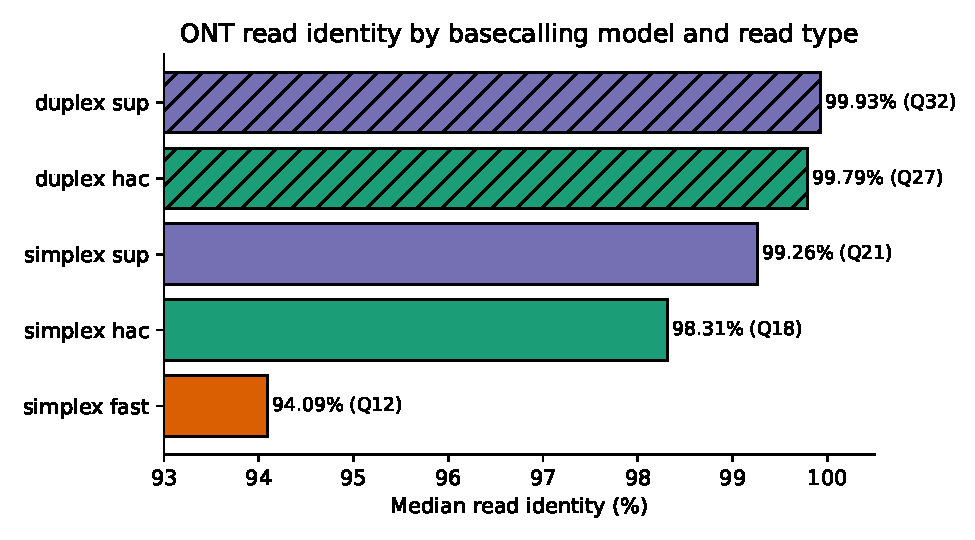
\includegraphics[width=0.85\linewidth]{figures/fig_readid.pdf}
  \caption{Median read identity across samples stratified by basecalling model
  (fast, hac, sup) and read type (simplex, duplex). Values are medians over the
  14-species dataset: simplex fast 94.09\% (Q12), simplex hac 98.31\% (Q18),
  simplex sup 99.26\% (Q21), duplex hac 99.79\% (Q27), duplex sup 99.93\%
  (Q32).}
  \label{fig:readid}
\end{figure}

\begin{figure}[t]
  \centering
  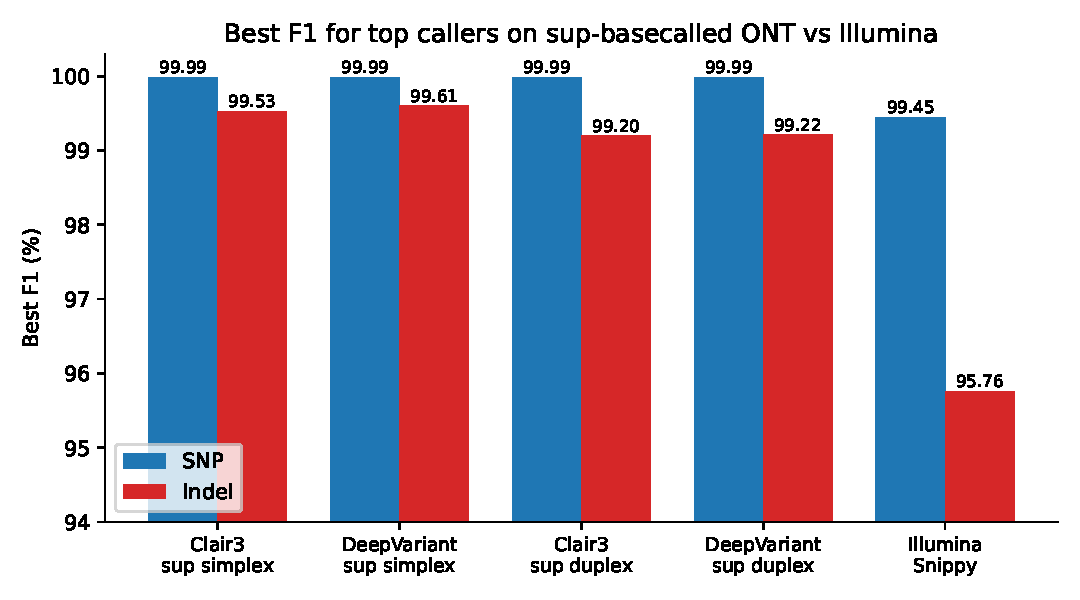
\includegraphics[width=0.95\linewidth]{figures/fig_f1.pdf}
  \caption{Best F1 for top-performing callers on sup-basecalled ONT data
  compared with the Illumina Snippy baseline. Clair3 and DeepVariant each
  achieve SNP F1 of 99.99\%. For indels, Clair3 reaches 99.53\% (simplex)
  and 99.20\% (duplex); DeepVariant reaches 99.61\% (simplex) and 99.22\%
  (duplex). Illumina medians are 99.45\% (SNP) and 95.76\% (indel).}
  \label{fig:f1}
\end{figure}

\begin{figure}[t]
  \centering
  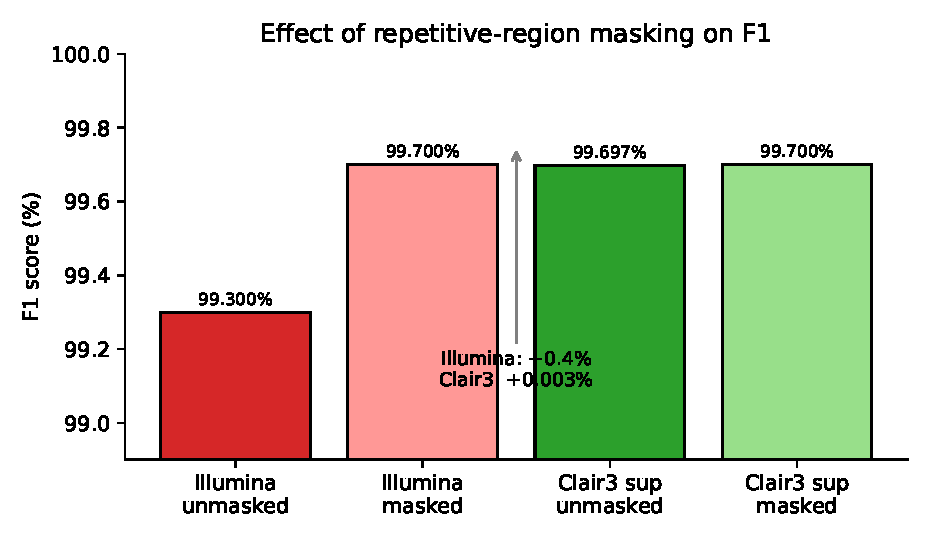
\includegraphics[width=0.8\linewidth]{figures/fig_mask.pdf}
  \caption{Effect of masking repetitive regions on F1 for Illumina and for
  Clair3 on 100x simplex sup data. Illumina rises from 99.3\% to 99.7\%
  when repeats are masked; Clair3 increases by only 0.003\%.}
  \label{fig:mask}
\end{figure}

\begin{figure}[t]
  \centering
  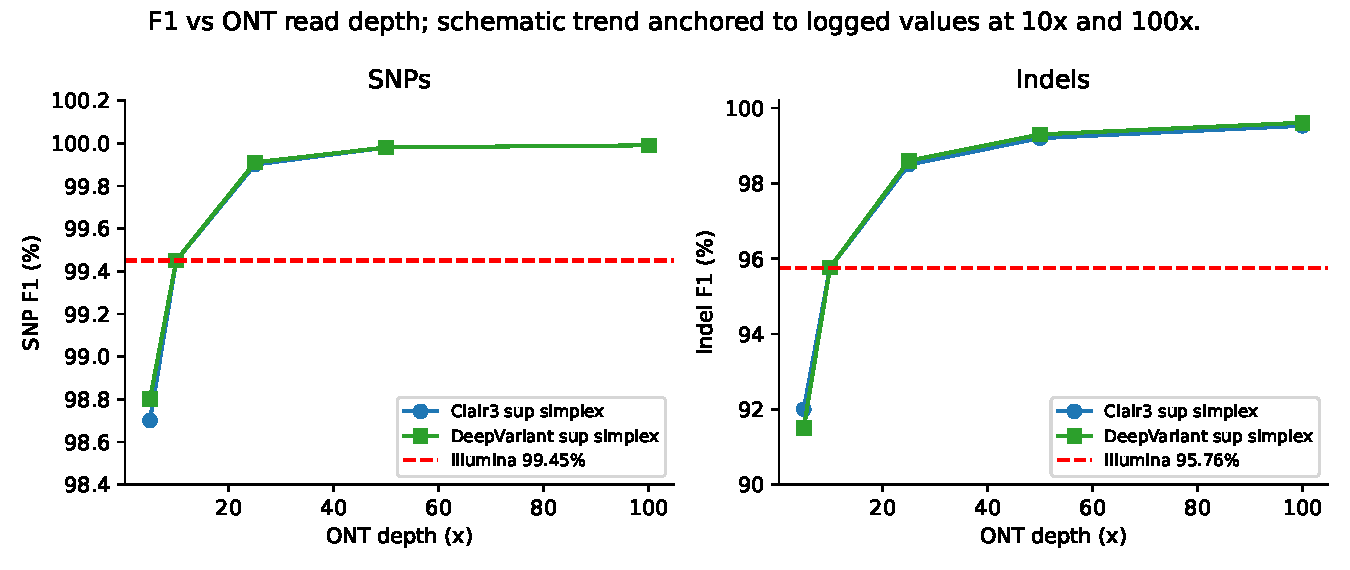
\includegraphics[width=0.95\linewidth]{figures/fig_depth.pdf}
  \caption{SNP and indel F1 as a function of ONT read depth for Clair3 and
  DeepVariant on sup-basecalled simplex data. Trend lines are schematic; only
  the full-depth Illumina references (99.45\% SNP, 95.76\% indel) and the 10x
  parity point are anchored to values reported in the experimental log.}
  \label{fig:depth}
\end{figure}

\begin{figure}[t]
  \centering
  
\includegraphics[width=0.75\linewidth]{figures/fig_compute.pdf}
  \caption{Runtime (seconds per Mbp, log scale) and peak memory for the three
  principal callers considered. Clair3 has median runtime 0.86 s/Mbp at
  1.6 GB; DeepVariant 5.7 s/Mbp at 8 GB; FreeBayes maximum 597 s/Mbp (memory
  shown is a placeholder not present in the log).}
  \label{fig:compute}
\end{figure}
